\section{Our Method}

\eat{
All events in a basketball game are performed in the same scene by the same set
of players. The only basis for differentiating these events is the action
pefromed by a small subset of players at a given time.  For instance, a
``steal" event is completely defined by the action of the player attempting to
pass the ball and the player stealing from him.  To understand such an event,
it is sufficient to observe only these players pariticipating in the event.

This motivates us to build a model which can reason about an event by focusing
on specific players during the different phases of the game.  Such a foucsing
mechanism would also provide valuable information about the game-state, making
the model more interpretable.
}

In this section, we describe our unified model for classifying events
and identifying the key players.


\subsection{Player detection and feature extraction}


We used AMT to annotate the location of all the players in a subset \KEVIN{HOW BIG?}
of the training data. We then trained a Multibox detector to detect players,
and ran this on all the training and test videos.  We kept all detections above
a confidence of 0.5 per frame; this resulted in between 0 and 10 (?) bounding
boxes per frame.  These detected player bounding boxs will also by the
multi-box model will be made available in the dataset.

\eat{
Given a set of basketball video clips, we first preprocess the clips to extract
player bounding boxes and features. We train a Multibox model \cite{} to detect
basketball players with bounding-box annotations collected on a subset of
training video frames. This model is then run on all frames of the training and
test videos to extract player bounding boxes.

A video clip $v$ is represented by a sequence of $D_f$ dimensional
frame-features $f_t$ extracted at each time-step $t$, as well as a set of $D_p$
dimensional player features $\mathcal{P}_t$ extracted from the player bounding
boxes at time $t$.

\begin{eqnarray}
  v & = & \left[ \left(f_1, \mathcal{P}_1\right), \dots,
\left(f_T, \mathcal{P}_T\right) \right]\;,\;\;f_t \in \mathbb{R}^{D_f} \\ \nonumber
\mathcal{P}_t & = & \{ p_{t1}, \dots, p_{t{P_t}} \}\;,\;\;p_{ti} \in \mathbb{R}^{D_p} \nonumber
\end{eqnarray}whre $P_t$ is the number of boxes at time $t$ and $T$ is the number of frames
in the video.
}

Each video-frame  is represented by a feature vector $f_t$, which is the activation
of the last fully connected layer of GoogLeNet \cite{} trained on ImageNet
\cite{}.  In addition, we compute spatially localized features.  In particular,
$p_{ti}$ contains both appearance and spatial information for the $i$'th
player bounding box in frame $t$. Similar to RCNN object detector\cite{},
the appearance features were extracted by feeding
the cropped and resized player region from the frame through GoogLeNet and
spatially pooling the response from a lower layer. The spatial feature
corresponds to a spatial histogram indicating the bounding box location.  
\VIGNESH{Should we include feature details here? I would prefere putting these
in more detail in the supp. material}

\subsection{Event classification}

Given $f_t$ and $p_{ti}$ for each frame $t$ from $1$ to $T$, our goal
is to train the model to classify the clip into one of 11 categories. As a side
effect of the way we construct our model, we will also be able to identify the
key player in each frame.

First we compute a global context feature for each frame, $h_t^f$, derived from
a bidirectional LSTM applied to the frame-level feature as shown in Fig.~\ref{fig:system_fig}.
This is a concatenation of the hidden states from the forward and reverse LSTM
components of a BLSTM and can be compactly represented as:
\[
h_t^f = \mbox{BLSTM}(h_{t-1}^f, h_{t+1}^f, f_t).
\]Please refer to Graves et al. \cite{Graves_2013} or the supp. material
for the full equations.

Next we use use a unidirectional LSTM to represent the state of the
game at time $t$:
\[
h_t^e = \mbox{LSTM}(h_{t-1}^e, h_t^f, a_t)
\]
where $a_t$ is a feature vector derived from the players, as we
describe below.
From this, we can predict the class label for the clip using $w_k^T
h_t^e$. We measure the loss as follows:
\begin{equation}
  L =   \frac{1}{2} \sum_{t=1}^T \sum_{k = 1}^K \max (0, 1 - y_k w_k^T h^e_t)^2
\end{equation} 
where $y_k$ is $1$ if the video belongs to class $k$,
else it is $-1$, and the weight vector corresponding to
class $k$ is denoted by $w_k$.

\subsection{Attention models}
\VIGNESH{I have added back my original motivation section for the attention model. I felt
that the section was descriptive and didn't motivate the method
sufficiently}
Unlike past attention models \cite{}, we need to attend to a different set of
features at each time-step. There are two key issues to address in this
setting.

First, although we have different set of detections in each frame, the player
detections can be connected across the frames through an object tracking
method. This could potentially lead to better feature representation of the
players.

Second, player attention depends on the state of the event and needs to evolve
with the event.  For instance, during the start of a ``free-throw" it is
important to attend to the player making the shot. However, towards the end of
the event the success or failure of the shot can be judged by observing the
person in posession of the ball.

With these issues in mind, we explore two models:
one without an object tracker and the other using an object tracker.


\noindent \textbf{Attention model without tracking}
Here, we treat the detections in each frame to be independent from other
frames.  This alows the model to be more flexible in switching attention
between players as the event progresses.  As we later observe empirically, this
leads to better interpretability.  Also, the model does not suffer from
tracking errors.

To compute $a_t$, we take a convex combination of the player features:
\begin{eqnarray} 
\label{eq:notrack}
  a_t^{notrack} & = & \sum_{i=1}^{N_t} \gamma_{ti}^{notrack} p_{ti} 
\\ \nonumber
  \gamma_{ti}^{notrack} & = & \text{softmax} \left(\phi\left(h^f_t, p_{ti}, h^e_{t-1}\right); \tau\right),
\end{eqnarray}
where $N_t$ is the number of detections in frame $t$,
and $\phi()$ is a 
multi layer perceptron $\phi$, similar to
\cite{Bahdnau_arxiv14}. 
$\tau$ is the softmax temperature parameter.
This model is illustrated in Figure~\ref{fig:model}(a).

\begin{figure*}[t!]
\begin{center}

   \subfigure[Attention without tracks]{
                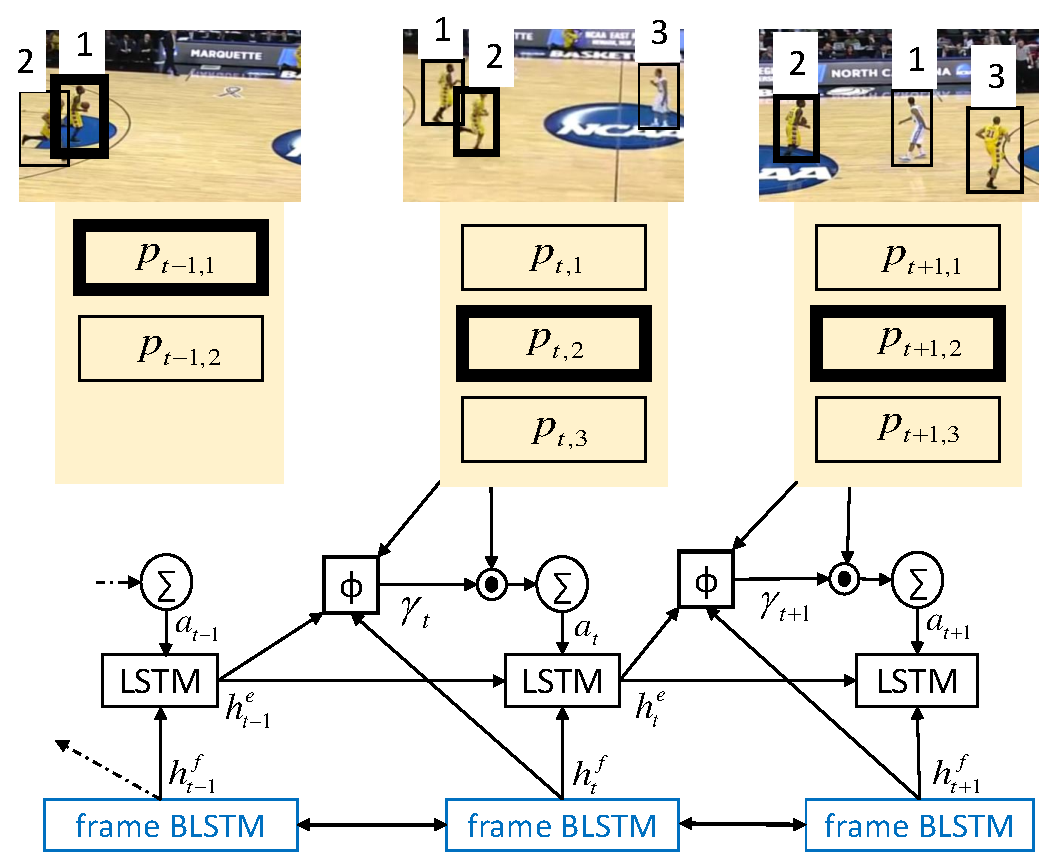
\includegraphics[width=3 in]{images/system_figure_2_cropped_v2.pdf}
                \label{fig:heatmap_ft}
    }
   \subfigure[Attention with tracks]{
                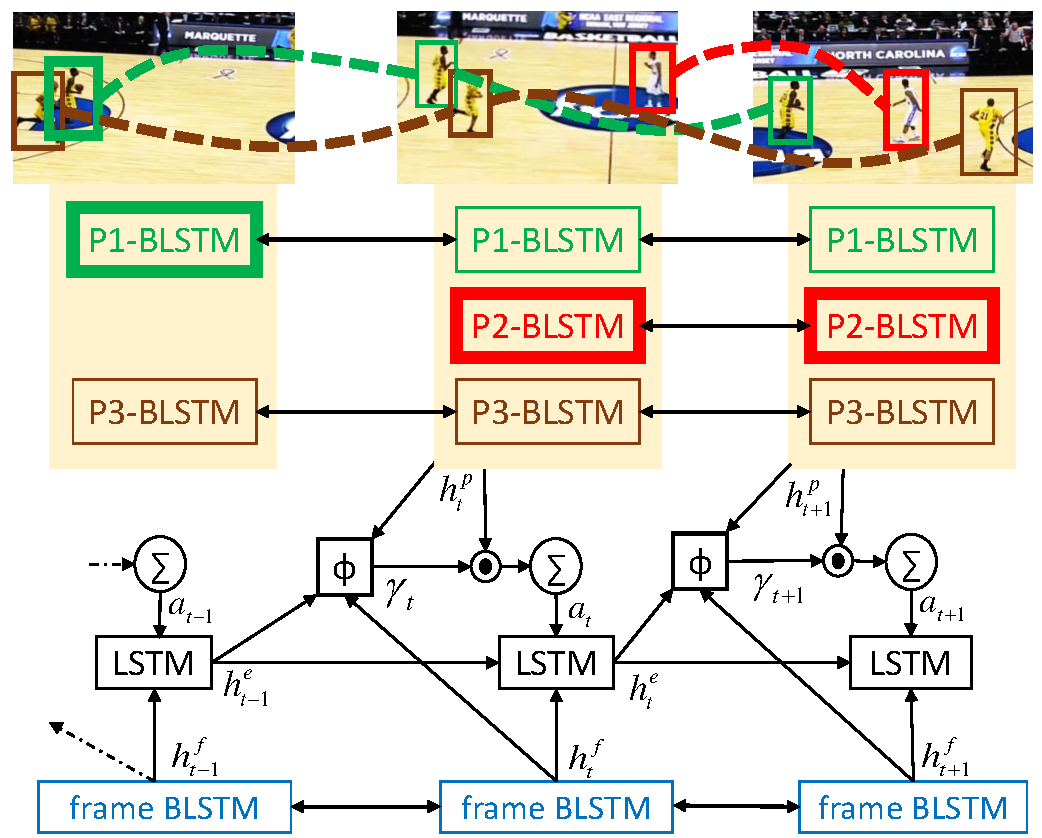
\includegraphics[width=3 in]{images/system_figure_1_cropped_v2.pdf}
                \label{fig:heatmap_lp}
    }
\end{center}
   \caption{Our attention models (a) without tracks and (b) with tracks are
   shown here. The variables in the model are explained in the methods
 section.
BLSTM stands for ``bidirection long short term memory''.
}
\label{fig:model}
\end{figure*}


\noindent \textbf{Attention model with tracking}

One potential weakness of the previous model is that the
player being attended to can change from frame to frame.
An alternative approach is to first associated detecitons
belonging to the same player into tracks using a standard
tracking method. We use a standard KLT tracker combined with
bipartite graph matching to perform the data association.
We then compute the attention scores as shown below:

\begin{eqnarray} 
\label{eq:track}
  a_t^{track} & = & \sum_{i=1}^{N_t} \gamma_{ti}^{track} p_{ti} 
\\ \nonumber
  \gamma_{ti}^{track} & = & \text{softmax} \left(\phi\left(h^f_t, h^p_{ti}, h^e_{t-1}\right); \tau\right),
\end{eqnarray}
where $h_{ti}^p$ is the latent represnetation of player $i$ in frame
$t$ computed using a BLSTM across tracks:
\[
  h_{ti}^p = \mbox{BLSTM}(h_{t-1,i}^p, h_{t+1,i}^p, p_{ti})
\]
This model is illustrated in Figure~\ref{fig:model}(b).
Below  we show that although this method gives slightly better
performance at event classification, it gives worse results for player
identification, because it is sensitive to tracking errors, and
is often unable to switch between players within an event.



\eat{
\subsection{Attention models}

Unlike past attention models \cite{}, we need to attend to a different set of
features at each time-step. There are two key issues to address in this
setting.

First, although we have different set of detections in each frame, the player
detections can be connected across the frames through an object tracking
method. This could potentially lead to better feature representation of the
players.

Second, player attention depends on the state of the event and needs to evolve
with the event.  For instance, during the start of a ``free-throw" it is
important to attend to the player making the shot. However, towards the end of
the event the success or failure of the shot can be judged by observing the
person in posession of the ball.

With these issues in mind, we explore two models:
one without an object tracker and the other using an object tracker.

\noindent \textbf{Player attention without tracking}
Here, we treat the detections in each frame to be independent from other
frames.  This alows the model to be more flexible in switching attention
between players as the event progresses.  As we later observe empirically, this
leads to better interpretability.  Also, the model does not suffer from
tracking errors.

At each time-step $t$, this model selects from the set of player features
$\mathcal{P}_t$. The attention is decided by a softmax weighting:

\begin{eqnarray} 
\label{eq:notrack}
  a_t & = & \sum_{i=1}^{P_t} \gamma_{ti} p_{ti} \\ \nonumber
  \gamma^{ti} & = & \text{softmax} \left(\phi\left(h^f_t, p_{ti}, h^e_{t-1}\right)\right; \tau),
\end{eqnarray}
where the attention value $\gamma_{ti}$ for the $i^{th}$ player
detection at $t$ is decided by a softmax over the player scores $e_{ti}$. This
score is obtained from a multi layer perceptron $\phi$, similar to
\cite{Bahdnau_arxiv14}. Refer to the supp. material for details.

\noindent \textbf{Player attention with tracking}
In this model, we first associate the detections across all the frames to
obtain tracks corresponding to each player in the video.  We use a
standard multi-object tracker with bipartite matching similar to
\cite{Veenman_PAMI2001} to obtain the tracks
Fig.\ref{fig:track_specific_model}.

The player-track is a temporal sequence representing the change in position and
appearance of the player with time.  We could use this to gain a better
representation for the player which incorporates temporal context from all
frames. Hence, we pass the features corresponding to the bounding box of the
track at each time-step through a BLSTM as shown in
Fig.~\ref{fig:track_specific_model}. Let the hidden state of this ``player"
BLSTM corresponding to the $k^{th}$ track be denoted by $h^p_{tk}$. Similar to
Eq.~\ref{eq:notrack}, the attention-weighted $a_t$ feature is given by:

\begin{eqnarray}
  a_t & = & \sum_{i=1}^{P_t} \gamma_{ti} h^p_{ti} \\ \nonumber
  \gamma^{ti} & = & \text{softmax} \left(\phi\left(h^f_t, h^p_{ti}, h^e_{t-1}\right); \tau\right),
\end{eqnarray}

While this provides a more consistent representation for the players across frames,
this model could suffer from wrong associations due to trakcing. This in turn makes
the interpretation of attention scores more difficult.


\subsection{LSTM event classifier}
Given a video $v$, we pass the frame-level features $f_t$ at time $t$ through a
Bidirectional Long Short-Term Memory (BLSTM) network. This helps in combining
contextual information from adjacent frames to provide a better frame
representation.  Let the hidden state of this BLSTM at time $t$ be denoted by
$h^f_t$.  This is the concatenated hidden state from both the forward and the
reverse LSTMS of the BLSTM. Refer to supp.  material for more details.

In order to attend to specific players in each frame, we pass the player features
through our attention model to generate an attention weighted player feature
$a_t$. The attention model is the main contribution of our work
and is explained in detail in the next section.

We feed the concatenated vector $[h^f_t, a_t]$ to a final event classification
LSTM, similar to the LRCN \cite{} model for video classification. Let
the hidden state of this LSTM at time $t$ be represented by $h^e_t$.  We then
train the model by minimizing the following one-vs-all hinge loss:

\begin{equation}
  L = \sum_{k = 1}^K \max (0, 1 - y_k w_k \cdot h^e_t)^2,
\end{equation} where $y_k$ is $1$ if the video belongs to class $k$,
else it is $-1$, and the weight vector corresponding to
class $k$ is denoted by $w_k$.
}
